\documentclass[aspectratio=169]{beamer}
\usetheme{Madrid}
\usepackage{graphicx}
\usepackage{booktabs}

\title{Branch Specialization in Attention}
\subtitle{Phase 1 Attention-Role Specialization Checkpoint}
\author{Research checkpoint}
\date{May 21, 2026}

\begin{document}

\begin{frame}
  \titlepage
\end{frame}

\begin{frame}{Current Question}
  \textbf{Question:} Do transformer heads have stable functional roles across seeds?

  \vspace{0.7em}
  Phase 0 showed weak universality in raw attention-score matrices:
  same-index similarity was low, but Hungarian matching recovered corresponding
  heads.

  \vspace{0.7em}
  Phase 1 now asks whether simple role proxies \(S(h,t)\) show the same pattern.
\end{frame}

\begin{frame}{Role Proxies}
  \begin{itemize}
    \item \textbf{BOS}: attention mass to token position 0.
    \item \textbf{Previous-token}: attention mass from position \(i\) to \(i-1\).
    \item \textbf{Repeat-match}: on synthetic repeated-token sequences
      \([x_1,\ldots,x_n,x_1,\ldots,x_n]\), attention from the second \(x_i\) to
      the first \(x_i\).
  \end{itemize}

  \vspace{0.6em}
  Scores are normalized across heads within a layer:
  \[
    S(h,t) = \frac{\mathrm{score}(h,t)}{\sum_{h'} \mathrm{score}(h',t)}
  \]
\end{frame}

\begin{frame}{Aggregate Cross-Seed Consistency}
  \begin{table}
    \centering
    \begin{tabular}{lrrr}
      \toprule
      Role & Raw & Aligned & Random \\
      \midrule
      BOS & 0.8317 & 0.8566 & 0.8310 \\
      Previous-token & 0.7531 & 0.8116 & 0.7531 \\
      Repeat-match & 0.5152 & 0.6191 & 0.5057 \\
      \bottomrule
    \end{tabular}
  \end{table}

  BOS is diffuse. Repeat-match has the clearest role-specific aligned-over-random signal.
\end{frame}

\begin{frame}{Repeat-Match Consistency}
  \centering
  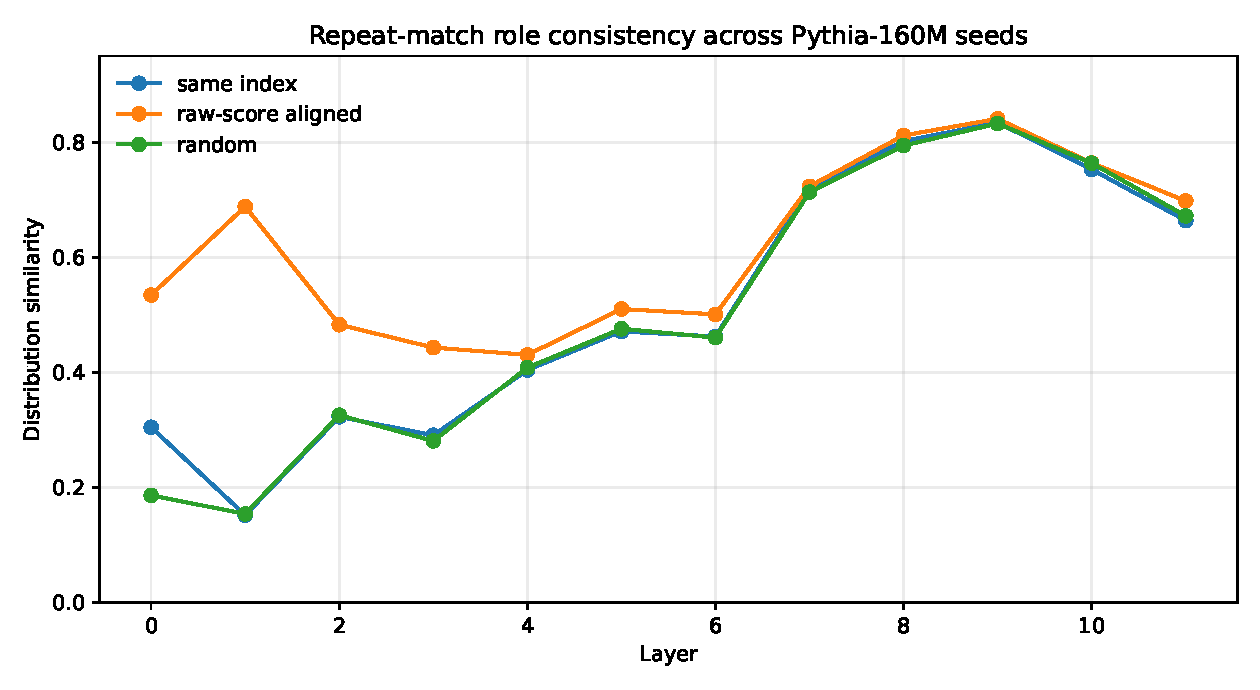
\includegraphics[width=0.88\linewidth]{figures/repeat_match_consistency.pdf}
\end{frame}

\begin{frame}{Role Concentration}
  \centering
  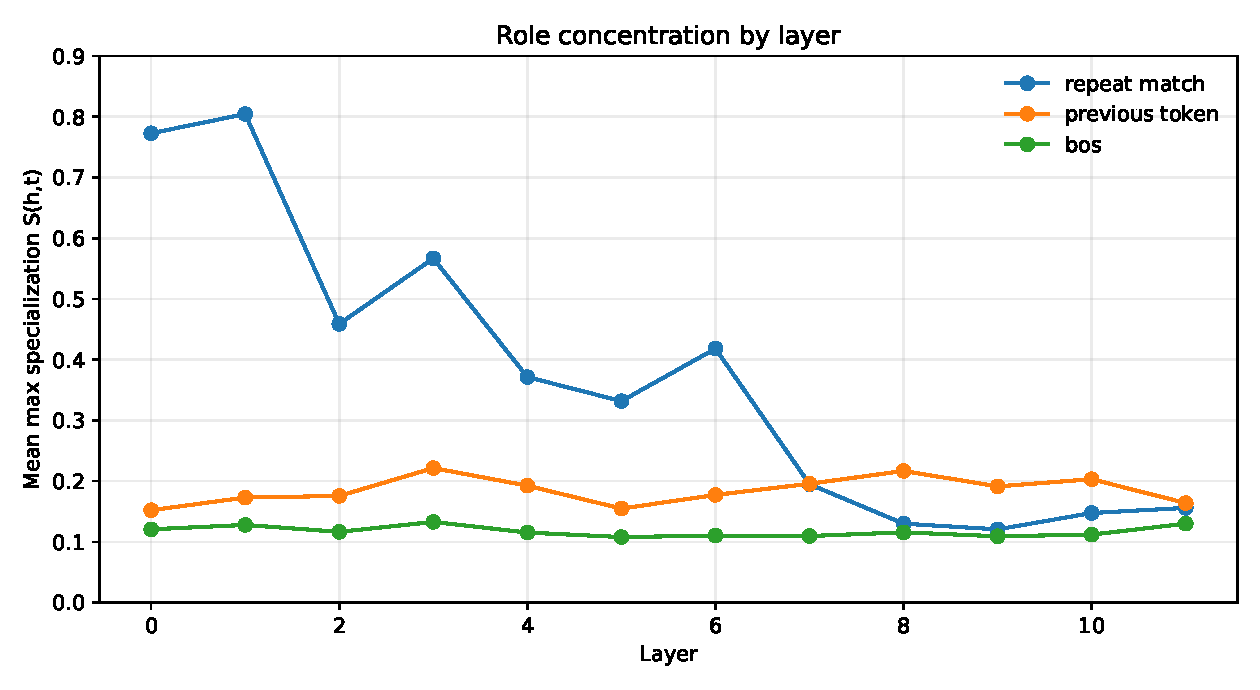
\includegraphics[width=0.88\linewidth]{figures/role_concentration.pdf}
\end{frame}

\begin{frame}{Top-Head Stability}
  \centering
  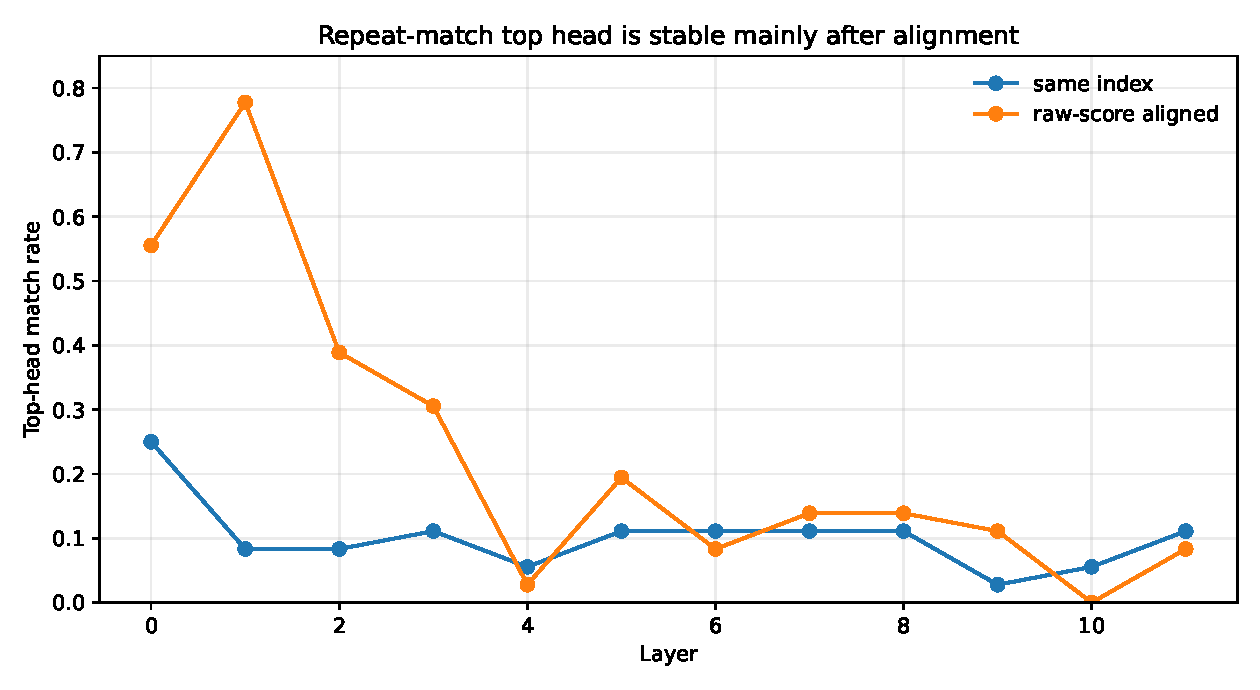
\includegraphics[width=0.88\linewidth]{figures/repeat_match_top_head_rate.pdf}
\end{frame}

\begin{frame}{Key Finding}
  Repeat-match is highly concentrated in early layers:

  \begin{table}
    \centering
    \begin{tabular}{lrrr}
      \toprule
      Role & Layer & Mean max \(S(h,t)\) & Effective heads \\
      \midrule
      Repeat-match & 0 & 0.7728 & 2.84 \\
      Repeat-match & 1 & 0.8045 & 2.26 \\
      Previous-token & 3 & 0.2215 & 10.31 \\
      BOS & 11 & 0.1300 & 10.60 \\
      \bottomrule
    \end{tabular}
  \end{table}

  This is the first clear branch-specialization-like signal in the project.
\end{frame}

\begin{frame}{Interpretation}
  \begin{itemize}
    \item A concentrated repeat-match attention role appears across Pythia-160M seeds.
    \item The responsible same-index head is unstable.
    \item Raw attention-score alignment recovers much stronger top-head agreement.
    \item This supports weak universality for a concrete role proxy, not just generic attention similarity.
  \end{itemize}
\end{frame}

\begin{frame}{Caveats}
  \begin{itemize}
    \item This is still an attention-pattern proxy, not causal patching.
    \item Repeat-match is induction-style, but not a full induction-copying behavioral test.
    \item BOS is not useful here because it is distributed and near random under permutation.
    \item Next step must test whether these heads causally affect repeated-token prediction.
  \end{itemize}
\end{frame}

\begin{frame}{Decision}
  \textbf{Continue with repeat-match / induction-style heads as the first causal target.}

  \vspace{0.8em}
  Next decisive experiment:
  \begin{itemize}
    \item identify top repeat-match heads in layers 0--1 for each seed;
    \item ablate those heads on repeated-token next-token prediction;
    \item compare against random heads and aligned corresponding heads.
  \end{itemize}
\end{frame}

\begin{frame}{Provenance}
  \begin{itemize}
    \item Script: \texttt{scripts/attention\_role\_specialization.py}
    \item Output: \texttt{results/phase1\_pythia160m\_attention\_role\_specialization}
    \item Report: \texttt{doc/phase1\_pythia160m\_attention\_role\_specialization.md}
    \item Alignment input: \texttt{results/phase0\_pythia160m\_seed1\_to\_9\_step143000\_raw\_scores/summary.json}
    \item Data copied into this deck folder under \texttt{data/}
  \end{itemize}
\end{frame}

\end{document}
